\documentclass[letterpaper,11pt,leqno]{article}
\usepackage{paper}
\usepackage{csquotes}
\usepackage{pgfplots}
\usepackage[l3]{csvsimple}
\pgfplotsset{compat=1.5}
\bibliographystyle{bibliography}

\usepackage{array}
\newcolumntype{L}[1]{>{\raggedright\let\newline\\\arraybackslash\hspace{0pt}}m{#1}}
\newcolumntype{C}[1]{>{\centering\let\newline\\\arraybackslash\hspace{0pt}}m{#1}}
\newcolumntype{R}[1]{>{\raggedleft\let\newline\\\arraybackslash\hspace{0pt}}m{#1}}

%
% Workaround for local / relative path problems in conjunction with reading csv file.
%
\newcommand{\csvpath}{/Users/dpfeifer/dev/intellij/genestrip-docs/genestrip-paper/}

% Enter paper title to populate PDF metadata:
%\hypersetup{pdftitle={MGenestrip: Efficient read classification, filtering and $k$-mer counting for selected groups of species}}

% Enter path to BibTeX file with references:
\newcommand{\bib}{bibliography.bib}

% Enter path to PDF file with figures:
%\newcommand{\pdf}{figures.pdf}

\begin{document}

% Enter title:
\title{Genestrip: Efficient read classification, filtering and $k$-mer counting for selected groups of organisms}

% Enter authors:
\author{Daniel Pfeifer (daniel.pfeifer@hs-heilbronn.de)
%
% Enter affiliations and acknowledgements:
\thanks{IT Faculty, Heilbronn University, Max-Planck-Str. 39, Heilbronn, 74081, Baden-Württemberg, Germany}}

% Enter date:
\date{January 2025}   

% Enter permanent URL (can be commented out):
%\available{https://github.com/pmichaillat/latex-paper}

\begin{titlepage}
\maketitle

% Enter abstract:
The consumption of computational resources is a significant burden in modern metagenomic analysis even when applying (unique) $k$-mer-counting. Genestrip overcomes this problem by focusing on small but freely selectable groups of organisms. Regarding the selected organisms, it produces results comparable to Kraken 1 and KrakenUniq but at a fraction of their required memory resources. Thus, mass data analysis may be performed even on small-sized PCs or servers. Moreover, Genestrip can be used to extremely reduce the size of sequence files for downstream steps without loss of relevant data regarding the selected organisms. We assess the usefulness, correctness and performance of Genestrip in the context of tick surveillance, ?? and ....

\end{titlepage}

\section{Introduction}

%Metagenomic analysis has become an extremely import field in bio informatics. 
With the availability of low cost and small-scale sequencing devices, metagenomic analysis will likely replace many established technologies for the detection and surveillance of specific groups of microorganisms. Related applications may affect various areas such as farming, ecology, food production and medicine. While sequencing devices have become ready for ubiquitous use, software tools for metagenomics still tend to be resource intensive and too hard to use for end users.

We present Genestrip, a new metagenomic tool based on $k$-mer matching and filtering that addresses the need for low resource consumption and ease of use. Genestrip is based on Java and can be run on all modern operating systems. ... competitive performance ...

\section{Background}\label{background}

To analyze large sets of reads, researchers use software tools based on $k$-mer matching and counting such as Kraken 1 \citep{kraken}, Kraken 2 \citep{kraken2} or KrakenUniq \citep{krakenUniq}. With regard to pathogen detection KrakenUniq is particularly suited because of its very low false positive rate but also because its efficiency, precision and sensitivity \citep{krakenUniq}.

In order to avoid false positive classifications of reads or mismatches of $k$-mers, all of these tools resort to very large databases, containing millions of encoded $k$-mers along with their respective taxons. A database is usually loaded entirely into main memory and consumes tens of gigabytes of space \footnote{See \url{https://benlangmead.github.io/aws-indexes/k2} for related Databases}. This requirement mandates specialized and expensive compute servers with very large main memory.

In recognition of this problem, KrakenUniq has been extended for database processing in chunks \citep{lowmemkraken}. However, ...

If only a smaller group of a few 100 species or strains is under consideration, then it seems promising to simply \emph{generate a smaller database that contains just the $k$-mers from respective genomes}. \emph{However, this very likely leads to many false positives} even when using KrakenUniq. The reason for this is that due to the evolutionary relationship of organisms, \emph{a large fraction of $k$-mers that belong to the genome of a species are unspecific} in a sense that they can as well be found in the genome other species not considered for analysis. Thus, when using too small a database, a read may be falsely assigned to a species because it consists of $k$-mers that \emph{also} belong to another species' genome that was not included in the database.
 
In order to enable a smaller database with no false positives emerging from this problem, Genestrip employs a \emph{two-phase} database generation process: During the \emph{entry phase}, all $k$-mers of genomes from selected organsisms are entered into the database on the basis of the RefSeq \citep{refseq} and optionally GenBank \citep{genbank}. During the \emph{update phase}, all stored $k$-mers from the database are checked against the genomes of all other organisms from the RefSeq belonging to the same (super-)kingdom. If a stored $k$-mer also occurs in another organism which is not part of the database, the $k$-mer's taxonomic identifier gets updated in the database and the least common ancestor's taxonomic identifier is entered instead. This prevents $k$-mers from being associated with one of selected organism even though they are unspecific.

Based on this approach Genestrip achieves very low memory footprints during analysis and a competitive $k$-mer matching and read classification performance. The actual $k$-mer counting results are similar to those of KrakenUniq \citep{krakenUniq} with regard to the selected organsisms. Much as KrakenUniq, Genestrip supports unique $k$-mer counting with exact counts but with very low memory overhead.

Although Genestrip supports read classification, the system's focus is on $k$-mer counting and associated statistics for several reasons:
\begin{itemize}
	\item Many modern sequencing devices produce long reads (with thousands of base pairs) but some with an error rate higher than 3\% per base pair \citep{nanoporeq, Delahaye:2021up}. Assuming an error of just 3\% per base pair, the chance of an erroneous $31$-mer is more than 60\%. This counters consistent read classification with high confidence --- particularly for long reads.
	\item Various, often configurable read classifications algorithms make respective results hard to compare and somewhat arbitrary \citep{metagenexp}.
	\item The authors of \cite{krakenUniq} show that statistics based on $k$-mer counting tend to be more predictive than read classification (Table 1 and Figure 3).
	\item Read classification incurs a considerable computational overhead at classification time.
\end{itemize}

\section{Methods}\label{methods}

\subsection{System Structure}

Genestrip's database generation mandates the setting of groups of organisms whose genomes will be exclusively represented in a resulting database. Users choose desired genuses, species and strains via a configuration file by listing respective taxonomic identifiers. If higher ranked taxonomic identifiers are entered, then \emph{all} of the descending organisms will be included and $k$-mers of their genomes will be added to the database accordingly. 

Genestrip generates a database for a selected group of organisms primarily via the 
reference genomes from the RefSeq \citep{refseq}.
To better handle the complexity of the generation process, we employ a goal-oriented approach in similarity to Make \citep{feldman1979make}. On access, each goal returns a file or an object in main memory. A goal is only executed if its result is not yet available. Goal execution may involve the access of other goals which turn, may trigger their execution. Respective goal dependencies are explicitly specified in terms of a directed acyclic graph. 

Figure \ref{f:goalgraph} depicts Genestrip's entire goal graph: Several goals (prefixed with \verb|d:|) revolve around downloading files from the RefSeq and other data from the NCBI. Several object goals (prefixed with \verb|o:|) load files and represent them as data structures in main memory for further processing. Most file goals (prefixed with \verb|f:|) write computational results to files.
Boxes with edged corners depict goals that can be executed directly via the command line. E.g., 
the goals \verb|match| and \verb|matchlr| are for fastq file analysis but they would trigger a respective database generation if the database file was missing.

\begin{figure}[h]%
\centering
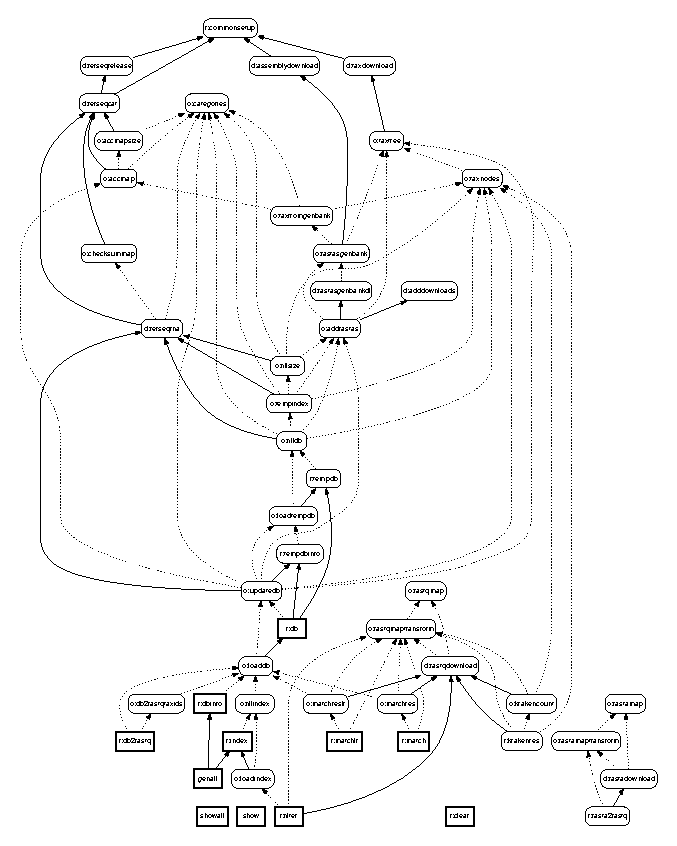
\includegraphics[width=14cm]{GoalGraph.eps}
\caption{Dependency Graph of Goals in Genestrip}\label{f:goalgraph}
\end{figure}
\clearpage

\subsection{Database and Filter Generation}

Genestrip stores a database primarily as a large array \verb|S| of sorted long values. Each long value encodes a $k$-mer from a reference genome of a selected organism. The default for $k$ is $31$ but other values are possible. A second array of the same size as \verb|S| encodes taxonomy identifiers for each $k$-mer in \verb|S|. During fastq file analysis, lookups in \verb|S| are performed via binary search.

At analysis time, A bit vector with same size as \verb|S| indicates which $k$-mers from \verb|S| were found at least once. This is sufficient for exact unique $k$-mer counting and is space-efficient, as it requires only about 1.6\% of additional memory with respect to \verb|S|.
An optional Bloom filter \citep{bloomfilter} also contains all stored $k$-mers. It is used by default at analysis time to check whether a certain $k$-mer is stored in \verb|S|. A negative result avoids a more expensive binary search in \verb|S| and therefore saves overall execution cost. 
Moreover, the parts of the NCBI taxonomy tree \citep{taxonomy} required at analysis time are included in 
the database. The taxonomy extract comprises entries for the selected organisms and all of its ancestors.

Besides $k$-mer matching and read classification, Genestrip also supports filtering of fastq files via a Bloom filter in similarity to \citep{biobloom}. When generated via the goal \verb|index|, the Bloom filter gets stored in separate file. The goal \verb|filter| loads the filter and processes fastq files accordingly. The standard configuration for the filtering process rewrites a read to the output if the read contains at least one $k$-mer that is recognized by the filter and thus, the read may belong to a selected organism.

Table \ref{goals} describes the most relevant goals for database generation in their typical execution order.

\begin{table}[h]
\centering
\begin{tabular}{l|p{10cm}}
 Goal Name & Description \\
  \hline
 \verb|fillsize| & Determines the maximum size of the database in number of $k$-mers by reading respective reference genome files and including genomes of selected organisms. It results in a conservative estimate as duplicates are double counted. \\
 \verb|tempindex| & Creates a Bloom filter filled with all $k$-mers of genomes of selected organisms. The Bloom filter's size is initially set via the result from \verb|fillsize|. As the Bloom filter avoids double counting, its final number of entries can serve as a more exact basis for the actual database size.\\
 \verb|filldb| & This \emph{entry phase} populates the database with all $k$-mers of genomes from selected organisms. The appropriate size of the database is a close but conservative estimate based on \verb|tempindex|.
  Duplicate $k$-mer entries are avoided via a Boom filter that tracks the already stored $k$-mers. Finally, the stored $k$-mers are sorted in order to enable binary search at analysis time but also for the goal \verb|updatedb| from below.\\
 \verb|updatedb| & This \emph{update phase} updates the populated database to account for common $k$-mers between organisms.
 \emph{All} genomes from the RefSeq belonging to a set of pre-configurable taxonomic (super-)kingdoms will be considered. This step ensures that a $k$-mer from a selected organisms obtains the correct taxonomic identifier as the $k$-mer may also occur in the genome of another organism (which might be represented in database or not). Concerning the finished database, the respective $k$-mer will be associated with the least common taxonomic ancestor of all organisms whose genomes contain the $k$-mer.\\
\end{tabular}
\caption{Description of Genestrip's most relevant goals for database generation}\label{goals}
\end{table}

\subsection{Statistical measures for $k$-mer counts}

Besides $k$-mer counts, unique $k$-mer counts and other results, Genestrip reports two novel, derived statistical measures -- \emph{the normalized $k$-mer count $k'_{t,f,d}$} and the \emph{$k$-mer consistency score} as described in the following.

Let $k_{t,f,d}$ be the number of $k$-mers for taxonomy identifier $t$ found in fastq file $f$ with respect to database $d$ and $u_{t,f,d}$ be the corresponding number of unique $k$-mers. Similarly $u_{t,d}$ is the number of (unique) $k$-mers for $t$ stored $d$, $k_f$ the total number of $k$-mers in $f$, $u_d$ the total number of (unique) $k$-mers stored in $d$ and so on.

Let $F$ be the set of analyzed fastq-files.
In order to compare $k_{t,f,d}$ between different files in $f \in F$ and potentially different databases $d$ or taxonomy identifiers $t$, we need to account for the a-priori bias caused by different file sizes $k_f$ and different numbers of stored $k$-mers $u_{t,d}$ of different taxonomy identifiers $t$ and different databases $d$.

We therefore consider the a-priori probability $p(t,f\ |\ d,F)$ which denotes the probability of $t$ to occur in $f$ given that (unique) $k$-mers of $t$ are stored in $d$. As this is an a-priori probability, we must assume independency between $t$ and any $g \in F$. As $f$ does not depend on $d$ this gives:
\[ p(t,f\ |\ d, F) = p(f\ |\ F) \cdot p(t\ |\ d) \approx k_{f} / \sum_{g \in F} k_{g} \cdot u_{t,d} / u_d\] 
We suggest a new measure -- \emph{the normalized $k$-mer count $k'_{t,f,d}$} that accounts for the a-priori bias:
\[ k'_{t,f,d} := c_{F} \cdot k_{t,f,d} /  k_{f} \cdot  u_d / u_{t,d} \approx k_{t,f,d} / p(t,f\ |\ d, F) \]
where $c_{F}$ captures the normalizing factor for $F$. As we don't depend on values in the range of $[0,1]$, we can simply set $c_{F} := 1$.

The \emph{the normalized $k$-mer count $k'_{t,f,d}$} accounts for the size of an organism's genome as represented in a database. This is relevant for abundance estimation via $k$-mer counting. As an example, assume a species $A$ has only got half as many specific $k$-mers in the database as another species $B$, so $u_{A,d} = 2 \cdot u_{B,d}$. Then, the same number of individual organisms for $A$ and $B$ in a sample would likely result in just half as many corresponding $k$-mers in a fastq file $f$ from shotgun sequencing, so $k_{A,f,d} \approx 2 \cdot k_{B,f,d}$. Still, the normalized $k$-mer count would yield $k'_{A,f,d} \approx k'_{B,f,d}$. 
%In other words, the normalized $k$-mer count accounts for different representation ratios between species in 
% Genestrip databases to allow for normalized abundance comparisons. 
	In analogous way, the normalized $k$-mer count also roughly accounts for differences in sequencing depths causing different values $k_{f}$ for different fastq files.\footnote{Note that the normalized $k$-mer count becomes less conclusive for abundance comparisons at higher taxonomic ranks $t$ because $u_{t,d}$ may result from a mix of organisms whose $k$-mers have all been pushed to $t$ as the least common ancestor. E.g., a $k$-mer under $t$ might be present in some but not all of the organisms under $t$ which skews $u_{t,d}$ as an estimation parameter in $k'_{t,f,d}$ with respect to abundance.}

Bracken \citep{lu2017bracken} follows a similar basic idea with respect to abundance estimation on the 
level of reads for Kraken. Still, Bracken's approach is significantly different from ours as it targets abundance estimation correction related to the specifics of the read classification algorithm behind Kraken.
  
Given $k_{t,f,d}$, the a-priori probability $p_u(t\ |\ k_{t,f,d})$ of a unique $k$-mer from $d$ belonging to $t$ to occur \emph{at least once} in $f$\ is approximately\footnote{The close but simplifying approximation being that all $k$-mers in $d$ belonging to $t$ are equally likely to be found in $f$.}:
\[ p_u(t\ |\ k_{t,f,d}) = 1 - (1 - 1/u_{t,d})^{k_{t,f,d}}\]
Therefore, the corresponding \emph{expected number of unique $k$-mers} $E_q$ is:
\[ E_q(k_{t,f,d},u_{t,d}) = u_{t,d} \cdot p_u(t\ |\ k_{t,f,d})\]
It is useful to compare $E_q$ with the actual count $u_{t,f,d}$: If these quantities divert too much from each other, then the consistency of the $k$-mer counting results for $t$ in $f$ should be questioned. If, on the other hand, these quantities are close, then this supports the consistency of the counting results. This justifies the following ratio as the \emph{$k$-mer consistency score}, which ideally is close to $1$:
\[ r(k_{t,f,d}, u_{t,f,d}) := u_{t,f,d} / E_q(k_{t,f,d},u_{t,d})\]
Table \ref{ebv} gives a real-world example where the $k$-mer consistency score shows to be useful.

\begin{table}[h]
\centering
\begin{tabular}{c|c|c|c|c|c|c}
$t$ & $u_{t,d}$ & $k_{t,f,d}$ & $u_{t,f,d}$ & $E_q(k_{t,f,d},u_{t,d})$ & $r(k_{t,f,d}, u_{t,f,d})$ & Coverage $u_{t,f,d} / u_{t,d}$  \\
  \hline
  10376 & $139502$ & $4151610$ & $120419$ & $139514$ & $0.8631$ & $0.8632$
\end{tabular}
\caption{Real extract of Genestrip analysis results for Human Gammaherpesvirus 4 from sequencing a human saliva sample: The $k$-mer count is over 34 times higher than the unique $k$-mer count but due to the short viral genome this is still close to the expectation as indicated by the $k$-mer consistency score of $0.8631$.}\label{ebv}
\end{table}

\footnote{A more mathematically sound approach is to consider the probability distribution 
$q(u_{t,f,d}\ |\ k_{t,f,d})$, i.e. the probability to obtain exactly $u_{t,f,d}$ unique $k$-mers for a given (non-unique) $k$-mer count of $k_{t,f,d}$ with  sampling with replacement as the underlying random process.
Interestingly, this distribution is non-trivial and has been investigated in \cite{Mendelson2016WhatIT}. The authors have shown that the distribution can be approximated by a normal distribution under most practically relevant conditions. Moreover, they confirm the expectation $E_q$ from above and give a formula for the variance $\sigma^2_q$ which in our case depends on $k_{t,f,d}$ and $u_{t,d}$. 
So, as an alternative consistency score one could set $r'(k_{t,f,d}, u_{t,f,d}) := f(u_{t,f,d}) / f(E_q)$,
where $f$ is the density of the normal distribution $\mathcal{N}(E_q,\sigma^2_q)$.
This relative density $r'$ ranges between $0$ and $1$ where $1$ is best and implies $u_{t,f,d} = E_q$.
Although mathematically sound, $r'$ did not appear useful with respect to $k$-mer counts because $\mathcal{N}(E_q,\sigma^2_q)$ tends to be extremely peaked and so, even small deviations from $E_q$ result in a $r' \approx 0$.}

%Expectation accounting for duplicate kmers in DB:
%Let $k_{t,d}(i)$ be the number of times a unique kmer $i$ occurs in the genome of $t$ with $1 \leq i \leq u_{t,d}$ and $\vec{k}_{t,d}$ the corresponding vector:
%\[ E_q(k_{t,f,d},\vec{k}_{t,d}) = \sum_{i = 1}^{u_{t,d}} k_{t,d}(i) \cdot (1 - (1 - 1/k_{t,d}(i))^{k_{t,f,d}}) \]

\subsection{$k$-mer Counting and Read Classification}


\subsection{Additional Features}

Genomic Dust, Removing $k$-mers from contaminating genomes. Read classification. Fully automated database builds.

\section{Results}\label{results}

\subsection{Accuracy}

To assess Genestrips's accuracy for $k$-mer counting, we compared its analysis results with 
corresponding results from KrakenUniq and Kraken2. We used the fastq files from \citep{nanoporeticks} where eight field-collected ticks were checked for tick-borne bacterial infections using Nanopore sequencing.
We generated an adequate Genestrip database covering well-known tick-transmitted bacteria as detailed in Line 1 of 
Table \ref{dbs}.

For comparison with KrakeUniq, we used with two different KrakenUniq databases: One commonly used, large database available online that includes all bacterial genomes from the RefSeq and more.
As an alternative, we created our own KrakenUniq database that covers the exact same genomes as the Genestrip database \enquote{Tick Borne} from Table \ref{dbs}. This database aims to show that a small KrakenUniq database covering just the organisms of interest, results in false positive $k$-mer counts and is therefore unsuitable for use.
Regarding Kraken2 we followed a similar procedure (see Table \ref{dbs}).

\begin{table}[h]
\centering
\begin{tabular}{c|p{2cm}|p{6cm}|r|r}
Type & Name & Description & Disk Size &$k$-mers\\
  \hline
G & Tick Borne & Genomes of a selection ??? species from the genuses Yersinia, Bartonella, Rickettsia, Anaplasma, Ehrlichia, Borrelia, Borreliella, Chlamydia, Mycoplasma, Malacoplasma, Mycoplasmoides and Metamycoplasma from the RefSeq (see taxlist for details)& 3 GB & 228 Mio. \\
K & Standard & From \url{https://benlangmead.github.io/aws-indexes/k2} (6/16/2022) & 377 GB & ?? \\
K & Tick Borne K & Same as for \enquote{Tick Borne} & ?? GB & ?? \\
K2 & Standard & From \url{https://benlangmead.github.io/aws-indexes/k2} (9/4/2024) & 80 GB & 15046 Mio. \\  
K2 & Tick Borne K2 & Same as for \enquote{Tick Borne} & ?? GB & ?? \\
\end{tabular}
\caption{Databases used for accuracy and performance comparisons (\enquote{G} means Genestrip, \enquote{K} means KrakenUniq, \enquote{K2} means Kraken2)}\label{dbs}
\end{table}

TODO: Correlation figures for $k$-mer counts, number of $k$-mers per database for selected species per rank (for tick borne K, tick borne and tick borne k2)

TODO: Same for grape vine fungi...

\subsection{Relevance of the Update Phase}

In order to validate the relevance of Genestrip's update phase we compared the contents of variants of the same Genestrip database. (See Section \ref{background} and Table \ref{goals} for background on the update phase.) In particular, we assessed, how the number of $k$-mers associated with each taxonomic identifier changes depending on the spectrum of genomes considered for the least common ancestor update. The database variants differed by having either
\begin{enumerate}
	\item no update phase (but just the entry phase), \label{noupdate}
	\item an update phase based \emph{exclusively} on the genomes from the entry phase, \label{minupdate}
	\item an update phase based on \emph{all} of the genomes of the corresponding taxonomic (super-)kingdom from the RefSeq.\label{completeupdate} 
\end{enumerate}
Table \ref{updaterelevance} documents respective results for ? different databases: Perhaps not surprisingly, the average percentage of $k$-mers that moved to higher taxonomic ranks is large when comparing variant \ref{noupdate} against variant \ref{minupdate} (see Column ($\bullet$)). However, a considerable amount of $k$-mers is also moved up when comparing variant \ref{minupdate} against variant \ref{completeupdate} (see Column($\circ$)). This indicates the importance of the update phase according to variant \ref{completeupdate} as otherwise, $k$-mer matches may lead to false positives at analysis time.

Figure \ref{tickchangekmers1} compares the results of fastq file analyses based on the \enquote{Tick Borne} database using variant \ref{minupdate} versus variant \ref{completeupdate}. We used the fastq files from \cite{nanoporeticks} and show the results for Tick 3 and Tick 6 as representative examples. The considerable changes in unique $k$-mer counts confirm that variant \ref{minupdate} is inferior for reliable $k$-mer counting due to false positives. Table \ref{topresultsticks} shows how the top ten hits under variant \ref{completeupdate} have changed under \ref{minupdate}: Major differences of unique $k$-mer counts and of respective frequency ranks solidify the design choice for Genestrip to employ an update phase according to \ref{completeupdate} as its default. Noteworthy, the results from Table \ref{topresultsticks} are also in line with the findings from \cite{nanoporeticks}.

\begin{table}[h]
\centering
\begin{tabular}{p{1.5cm}|p{1.5cm}|R{1.3cm}|R{1.3cm}|R{1.5cm}|r|R{1.5cm}|R{1.5cm}}
Database Name & (Super-)Kingdom & Genuses With at Least One Species & Species & Strains & $k$-mers & ($\bullet$) \newline \% of $k$-mers moved up &  ($\circ$) \newline \% of $k$-mers moved up \\
  \hline
  \hline
 Tick Borne & Bacteria & 13 & 95 & 574 & 226765827 & & 17.75 \\
  \hline
 Grape Vine Fungus & Fungal & ?? & ??
\end{tabular}
\caption{Change of taxonomic identifiers for $k$-mers in Genestrip databases due to the update phase: The comparison of database variants is between \\
(1) \ref{noupdate} versus \ref{minupdate}, i.e. \emph{no} update phase (but just the entry phase) versus an update phase based \emph{exclusively} on the genomes from the entry phase or else, \\
(2)	\ref{minupdate} versus \ref{completeupdate}, i.e. an update phase based \emph{exclusively} on the genomes from the entry phase versus \emph{all} of the genomes of the corresponding taxonomic (super-)kingdom from the RefSeq.}
\label{updaterelevance}
\end{table}

\begin{figure}[h]%
\centering
\begin{tikzpicture}
\begin{axis}[
title=Tick 3,
xlabel={unique $k$-mers, variant \ref{minupdate}},
ylabel={unique $k$-mers, variant \ref{completeupdate}},
xmode=log,
ymode=log,
width = 0.6\textwidth,
height = 0.6\textwidth
]
\addplot+ [only marks,mark size=1pt]
table[col sep=semicolon, header=true, x = {kmers 2}, y = {kmers 1}] {\csvpath results/chronicb/tick3_ukmer_scatter.csv};
\end{axis}
\end{tikzpicture}

\begin{tikzpicture}
\begin{axis}[
title=Tick 6,
xlabel={unique $k$-mers, variant \ref{minupdate}},
ylabel={unique $k$-mers, variant \ref{completeupdate}},
xmode=log,
ymode=log,
width = 0.6\textwidth,
height = 0.6\textwidth
]
\addplot+ [only marks,mark size=1pt]
table[col sep=semicolon, header=true, x = {kmers 2}, y = {kmers 1}] {\csvpath results/chronicb/tick6_ukmer_scatter.csv};
\end{axis}
\end{tikzpicture}
\caption{Scatter plots of unique $k$-mers for fastq files from \cite{nanoporeticks} analyzed using Genestrip and the variants \ref{minupdate} versus \ref{completeupdate} of the \enquote{Tick Borne} database on logarithmic scales. Each datapoint represents a taxonomic identifier with counts greater zero for at least one variant.}\label{tickchangekmers1}
\end{figure}

\begin{table}[h]
\small 
\centering
\begin{tabular}{C{2.1cm}|c|R{1.6cm}|R{1.6cm}|R{1.5cm}|R{1.5cm}|R{1.5cm}}
Name & Tax. Id. & Unique $k$-mers under Variant \ref{minupdate} & Resulting Rank under Variant \ref{minupdate} & Unique $k$-mers under Variant \ref{completeupdate} & Resulting Rank under Variant \ref{completeupdate} & Unique $k$-mer Change from \ref{minupdate} to  \ref{completeupdate} in \% \\
\hline
\hline
\textbf{Tick 3} \\
\hline
\csvreader[separator=semicolon]{\csvpath results/chronicb/tick3_kmer_changes.csv}{}{\csvcoliii & \csvcolii & \csvcolv & \csvcoliv & \csvcolvi & \csvcolvii & \csvcolviii \\   \hline }	
\textbf{Tick 6} \\
\hline
\csvreader[separator=semicolon]{\csvpath results/chronicb/tick6_kmer_changes.csv}{}{\csvcoliii & \csvcolii & \csvcoliv & \csvcolv & \csvcolvi & \csvcolvii & \csvcolviii \\   \hline }	
\end{tabular}
\caption{Change of unique $k$-mer counts for top ten hits of Tick 3 and Tick 6 from \cite{nanoporeticks} using Genestrip and the variants \ref{minupdate} versus \ref{completeupdate} of the \enquote{Tick Borne} database}\label{topresultsticks}
\end{table}

\subsection{Performance}

To assess Genestrips's performance for $k$-mer counting, we compared its analysis time and memory use with 
corresponding analysis runs using KrakenUniq and Kraken2.

...

\section{Discussion}\label{discussion}

\section{Availability}
Tell where to download all of the software...

\clearpage
\bibliography{bibliography}

\end{document}